% `template.tex', a bare-bones example employing the AIAA class.
%
% For a more advanced example that makes use of several third-party
% LaTeX packages, see `advanced_example.tex', but please read the
% Known Problems section of the users manual first.
%
% Typical processing for PostScript (PS) output:
%
%  latex template
%  latex template   (repeat as needed to resolve references)
%
%  xdvi template    (onscreen draft display)
%  dvips template   (postscript)
%  gv template.ps   (onscreen display)
%  lpr template.ps  (hardcopy)
%
% With the above, only Encapsulated PostScript (EPS) images can be used.
%
% Typical processing for Portable Document Format (PDF) output:
%
%  pdflatex template
%  pdflatex template      (repeat as needed to resolve references)
%
%  acroread template.pdf  (onscreen display)
%
% If you have EPS figures, you will need to use the epstopdf script
% to convert them to PDF because PDF is a limmited subset of EPS.
% pdflatex accepts a variety of other image formats such as JPG, TIF,
% PNG, and so forth -- check the documentation for your version.
%
% If you do *not* specify suffixes when using the graphicx package's
% \includegraphics command, latex and pdflatex will automatically select
% the appropriate figure format from those available.  This allows you
% to produce PS and PDF output from the same LaTeX source file.
%
% To generate a large format (e.g., 11"x17") PostScript copy for editing
% purposes, use
%
%  dvips -x 1467 -O -0.65in,0.85in -t tabloid template
%
% For further details and support, read the Users Manual, aiaa.pdf.


% Try to reduce the number of latex support calls from people who
% don't read the included documentation.
%
\typeout{}\typeout{If latex fails to find aiaa-tc, read the README file!}
%


\documentclass[]{aiaa-tc}% insert '[draft]' option to show overfull boxes
\usepackage{amsmath}								%For mathematical typesetting
\usepackage{amssymb}								%For mathematical typesetting
\usepackage{listings}								%Code formatting
\usepackage{wrapfig}

 \title{A High-Order Conservative Eulerian Simulation Method for Vortex Dominated Flows}

 \author{
Joshua J. Bevan\thanks{Graduate Student, Department of Mechanical Engineering.}
\ and David J. Willis\thanks{Associate Professor, Department of Mechanical Engineering, Senior Member AIAA.}\\
{\normalsize\itshape
 University of Massachusetts Lowell, Lowell, Massachusetts, 01854, U.S.A.}\\
 }

 % Data used by 'handcarry' option if invoked
 \AIAApapernumber{YEAR-NUMBER}
 \AIAAconference{Conference Name, Date, and Location}
 \AIAAcopyright{\AIAAcopyrightD{YEAR}}

 % Define commands to assure consistent treatment throughout document
 \newcommand{\eqnref}[1]{(\ref{#1})}
 \newcommand{\class}[1]{\texttt{#1}}
 \newcommand{\package}[1]{\texttt{#1}}
 \newcommand{\file}[1]{\texttt{#1}}
 \newcommand{\BibTeX}{\textsc{Bib}\TeX}

\newcommand{\be}{\begin{equation}}
\newcommand{\ben}[1]{\begin{equation}\label{#1}}
\newcommand{\ee}{\end{equation}}
\newcommand{\aomega}{\overset{\sim}{\omega}}				%Approximate omega

\begin{document}

\maketitle

%============================================================
\begin{abstract}
A high-order, conservative Eulerian method is presented for the simulation of vortex dominated inviscid fluid flows. The primitive variable incompressible Euler equations are recast in the velocity-vorticity form to explicitly enforce conservation of vorticity. The advection of the vorticity is then calculated via a two-step process: the velocity field is determined by evaluation of the Biot-Savart integral, and then a line-based discontinuous Galerkin (DG) Eulerian spatial discretization scheme is applied to accurately advect the vorticity field. The accuracy and convergence of this method was examined for test cases where an analytical solution exists, as well as more challenging test cases which lack an analytical solution. The convergence rate behavior is chiefly controlled by the error in the calculated velocity field. Velocity errors are due to two factors: the approximation of the Biot-Savart integral with a desingularized form, and reduced quadrature convergence for the nearly singular integral. Solver parameters were chosen to balance these two effects resulting in nearly optimal convergence of the overall method in the analytical test, and high-order convergence in the qualitative test case.
\end{abstract}

%============================================================
%\section*{Nomenclature}

%\begin{tabbing}
%  XXX \= \kill% this line sets tab stop
%  $J$ \> Jacobian Matrix \\
%  $f$ \> Residual value vector \\
%  $x$ \> Variable value vector \\
%  $F$ \> Force, N \\
%  $m$ \> Mass, kg \\
%  $\Delta x$ \> Variable displacement vector \\
%  $\alpha$ \> Acceleration, m/s\textsuperscript{2} \\[5pt]
%  \textit{Subscript}\\
%  $i$ \> Variable number \\
% \end{tabbing}

%============================================================
\section{Introduction}
Direct solution of Navier-Stokes is impractical for many fluid problems and where possible simplifications should be made; one such possibility is for vortex dominated flows. It is possible to recast Navier-Stokes from a primitive variable form ($u,v,p$) to a velocity-vorticity ($u,v,\omega$) form. This has several advantages: explicit conservation of vorticity, elimination of pressure terms (for incompressible flows), and reduction of required simulated degrees of freedom to just those that form the vorticity support.

Many vortex based simulation techniques use a Lagrangian approach to discretize the vorticity into a set of vortex particles\cite{Point4}, lines\cite{Line4}, sheets\cite{Sheet1}, or volumes\cite{Volumes1}. This is a natural approach to take given the material nature of the vorticity due to Helmholtz and Kelvin's theorems.

%Lagrangian codes
The velocity field due to the vorticity is calculated from solving the Poisson problem \cite{MiscMeth1}, or through inversion of the Poisson problem via evaluation of the Biot-Savart integral \cite{Saffman1992}. There are several challenges with evaluation of the velocity: boundary conditions in the Poisson solution method, and singularities in the Biot-Savart volume integral method. Typically Lagrangian point vortex codes must de-singularize the kernel \cite{Rosenhead1930,Moore1972}. Direct summation for the velocity field has a $\mathcal{O}(N^2)$ complexity. Tree-codes \cite{LindsayKrasny2001} and Fast Multipole Methods (FMM) \cite{Strain1997} are ways of achieving a more efficient calculation.

Lagrangian point methods present several problems. Point disorganization can occur as the fluid evolves, this typically requires temporary meshing to recondition the discretization. This has been handled with various methods; recalculation of the quadrature weights at each time step \cite{Remesh2,Remesh3}, regridding/rezoning \cite{Remesh4}, and remeshing \cite{Remesh5} among them. Additionally, most Lagrangian approaches are limited to low order; careful point locations must be chosen and maintained through frequent remeshing etc. in order to achieve high-order convergence \cite{Strain1997}.

%Existing Eulerian codes
In comparison, Eulerian approaches to vortex methods tend to be less common. Work has been done for viscous flows with solid bodies; both stationary \cite{MiscMeth3} and moving \cite{MiscMeth2}. Both of these solve the streamfunction-vorticity formulation, not the velocity-vorticity formulation. The velocity-vorticity formulation has been solved by an Eulerian approach by others \cite{MiscMeth4}. A notable example of an Eulerian approach to the velocity-vorticity formulation is the work of Brown et al. \cite{Brown2000} who adapted the velocity-vorticity approach to a low order Finite Volume (FV) solver. Later they were able to extend their method to be accelerated via a FMM \cite{Brown2004}. However, like most FV approaches, to extend to high order solution approximations requires extended stencils that ultimately limit the geometrical freedom of the mesh. Steinhoff et al. also used an Eulerian approach, but solved a modified form of the inviscid Euler equations with ``vorticity confinement'' rather than the velocity-vorticity equation \cite{SteinhoffUnderhill1994}.

%Choice of present method
The desire to resolve fine vortical structures motivates the need for a high order solver. Considering the challenges associated with achieving a high order Lagrangian method and the success of Brown et al.'s low order method, a high order Eulerian vorticity-velocity method would seem to be a possible choice. This leaves the choice of a spatial discretization.

Finite difference methods suffer from similar problems as FV with extended stencils, as well as not being explicitly conservative. A finite element approach is ill-suited to the hyperbolic nature of vorticity advection. Spectral methods are promising, but for sparse vorticity domains are less-efficient due to the global support of the harmonic bases. However, discontinuous Galerkin (DG) methods \cite{HestWar} are a natural choice; they are conservative, able to take advantage of vorticity sparseness, are well-suited to handle advection via intelligent choice of a numerical flux function, and have bases with local/compact support.

For domains free of impinging bodies a hexahedral mesh with a tensor product grid of interpolation points is convenient to implement. This permits the use of a line-DG \cite{Persson2013} approach that considerably simplifies multi-dimensional cases by allowing reuse of 1D methods. Initial investigation done in 2D permits evaluation of whether the method is practical, as well as to limit solution times to those that are reasonable on a workstation. It also has the advantage of removing the vortex stretching term and reducing the vorticity to a scalar. The resultant partial differential equation (PDE) takes on the familiar form of a scalar conservation law. To maintain maximum flexibility for investigative purposes and to remove as much approximation error as possible the velocity field for validation of the underlying method is calculated via direct evaluation of the Biot-Savart integral.

%============================================================
\section{Governing Equations and Discretization}
\subsection{Velocity-Vorticity Formulation}
The Navier-Stokes momentum equation is
 \be \rho \left(\frac{\partial \mathbf{u}}{\partial t} + \mathbf{u} \cdot \nabla \mathbf{u} \right) = -\nabla p + \mu \nabla^2 \mathbf u + \tfrac13 \, \mu \nabla (\nabla\cdot\mathbf{u}) \ee
where $u$ is the velocity field, $p$ is the pressure, and $\rho$ is the density. If we restrict ourselves to incompressible flows and define the quantity \textit{vorticity} as
\be \mathbf{\omega} = \nabla \times \mathbf{u} \ee
then the traditional form of the Navier-Stokes equations can be recast:
\ben{VV3D} \frac{\partial \omega}{\partial t} +  \mathbf{u} \cdot \nabla \omega - \omega \cdot \nabla  \mathbf{u} = S(x,t)\ee
We are interested in inviscid flows, so we collect viscous generation of vorticity in $S$ and permit it to be externally specified if necessary.

For 2-D distributions of vorticity, several simplifications can be made. The originally vectorial vorticity becomes a scalar quantity, all vorticity is directed normal to the plane. As a result, the vortex stretching term in  Eqn.\,\eqref{VV3D} becomes zero. The only non-zero component of $\omega$ is in the z-direction, however the gradient of the velocity field is zero in the z-direction, so the product is therefore zero. The result is
\ben{VV2D} \frac{\partial \omega}{\partial t} + u \cdot \nabla \omega = S(x,t)\ee
or if instead the second term is expressed in terms of the flux of the vorticity (where $f_i(\omega)=u_i\,\omega$):
\ben{VV2DB} \frac{\partial \omega}{\partial t} + \frac{\partial f}{\partial x_i}= S(x,t)\ee

 For an incompressible 2D or 3D flow we can relate the velocity and vorticity by:
\be \nabla^2 u = -\nabla \times \omega \ee
If inverted, the Biot-Savart integral is obtained
\ben{BS} u(x^*) = \int_\Omega K(x^*,x) \times \omega(x) dx \ee
where $x^*$ is the point we wish to evaluate the velocity, $x$ is the coordinate in regions of non-zero vorticity, and $K(x^*,x)$ is the singular Biot-Savart kernel \cite{BealeMajda}
\ben{BSkern} K(x^*,x) = \frac{-1}{2 \pi} \frac{x^*-x}{|x^*-x|^2} \ee

The high-order Eulerian approach taken here means that while the Biot-Savart integral converges, a singularity is always present within any of the extended vorticity patches thanks to self-influence. Conceptually this doesn't present an impossible problem, the integral \textit{does} converge in an analytical sense; practically speaking however a singularity may cause numerical integration procedures to diverge, or at the very least converge quite slowly. The approach taken by Brown \cite{Brown2004} was to use the Rosenhead-Moore kernel, choosing a core size such that the maximum velocity occurred on the face of the finite volume unit. This can be constructed \textit{a priori} because the vorticity is taken as constant across the volume, as is typical in a FV approach. If the vorticity is spatially varying however, the choice of core size is more troublesome.

One may attempt to desingularize the Biot-Savart kernel by introducing a core function $\eta(^z/_{\delta})$, with characteristic cutoff radius $\delta$. Traditionally the core function is convolved with the Biot-Savart kernel to yield a desingularized kernel $K_{\delta}$.
\ben{DesingBS} K*\eta(r) = K_{\delta} \ee

The choice of a core function and a characteristic radius has important implications on the accuracy and convergence of a Lagrangian point vortex method. Choosing a cutoff radius too small and there is insufficient smoothing, too large and the vorticity discretization is spatially smeared. In a Lagrangian method the convolution with a core function has a physical heuristic: the point vortex is replaced by a finite size vortex blob described by $\eta(r)$, with characteristic radius $\delta$. 

In contrast in the present method the core function is a means to an end; attempting to numerically integrate the singular Biot-Savart integral will result in spurious values, so the desingularized kernel is used as an approximation. A number of kernels can be chosen in a Lagrangian method, we found the following kernel\cite{WL} generally had the lowest approximation error for our purposes:
\ben{PSkern0}  K_{spectral}= \frac{z}{2 \pi |z|^2} (1-J_0(\frac{z}{\delta})) \ee
where we have substituted $z=x^*-x$, and $J_\alpha$ is a Bessel function of the first kind.

%---------
\subsection{Discontinuous Galerkin Spatial Discretization}
In order to solve Eqn.\,\eqref{VV2D} we adopt a method-of-lines approach \cite{RKDG}. We will first spatially discretize the system to obtain the semi-discrete system, then we use an explicit time discretization method to march forward in time. Note that Eqn.\,\eqref{VV2D} has the form of a scalar conservation law, with $\omega$ being the conserved quantity. The velocity field that advects the conserved quantity has been calculated by evaluation of the Biot-Savart integral for the current timestep.

We use a standard nodal DG formulation\cite{HestWar} for the 1D problem, resulting in the variational form defined on a particular element:
\be \int_\Omega \frac{\partial \aomega}{\partial t} \, \phi_j \;dx + \int_\Omega \frac{\partial f(\aomega)}{\partial x} \, \phi_j \;dx = 0 \quad\mbox{for all}\; j\ee
where $\aomega$ is the solution approximation for the vorticity, and $\phi_j$ is the $j^{th}$ test function.  Both the solution approximation bases and the test functions are apart of the same polynomial vector space.

We take the set of Lagrange polynomials as the basis for our polynomial vector space. The interpolatory property of the Lagrange basis means that $\ell_i(x_j) = \delta_{ij}$, so that the value of the function at the interpolation points forms the expansion coefficients. Therefore the local Mth order approximation to vorticity takes the form:
\be \omega(x,t) \approx \aomega(x,t) = \sum_{i=0}^M a_i(t)\psi_i(x)\ee
where $a_i$ is the value of the vorticity interpolation at the $i^{th}$ node, and $\psi_i$ is the $i^{th}$ solution approximation basis.

The spatial discretization thus described only concerns the solution within an element. Continuity across elements is not enforced in DG, the solution is multiply defined at coincident nodes from neighboring elements. To recover the global solution, flux functions are usually employed to couple local elemental solutions to one another. We use an upwind flux, where defining the average as $\{\!\{\omega^+\}\!\} = \frac{\omega^++\omega^-}{2}$ and the jump as $[[\omega]]=\omega^+-\omega^-$ \cite{HestWar}, yields
\be \hat{f}_{upwind}(x^+,x^-)=u\{\!\{\aomega\}\!\} + \frac{|u|}{2}[[\aomega]]\ee

Continuing to follow a standard nodal DG approach and substitution of these choices of bases functions and flux functions yields the elemental form:
\ben{DGtemp2} \frac{\Delta x}{2}	\sum_{i=0}^M \left[ \frac{d a_i}{dt}	\int_{-1}^{1}\psi_i  \, \phi_j \;dX \right]
+\hat{f}\phi_j \Big|^{x_R}_{x_L} 
- \int_{-1}^{1} f(\aomega) \, \frac{d \phi_j}{dX} \;dX = 0 \ee
where $x_R$ and $x_L$ are the element bounds, we have mapped to a computational element $X \in [-1, 1]$ via the mapping $X=G(x)=\frac{2(x-x_L)}{\Delta x}+1$, and $\Delta x = x_R - x_L$ is the element size.

Thus far only a 1D solution has been discussed. The 2D solution basis is formed from the tensor product of two orthogonal 1D solutions, each along a coordinate axis. An important consequence of the tensor basis and hexahedral mesh is that the two basis directions are not coupled except at the interpolation nodes at the intersection of each direction's basis. This is the central idea in the line-DG \cite{Persson2013} approach, a 2D problem is transformed into two 1D problems of the form of Eqn.\,\eqref{DGtemp2}. The 2D time evolution of the overall system is the linear combination of the 1D evolutions; notably the instantaneous rate of change of a particular node is the sum of the rates from each direction.

We can now use the developed 1D basis in a tensor product to form our 2D basis
\be f(x,y) \approx \left[\sum_{t=0}^M z_t \ell_t(y) \right] \times \left[ \sum_{s=0}^M z_s \ell_s(x) \right] = \sum_{t=0}^M \sum_{s=0}^M z_{st} \ell_t \ell_s =  \sum_{t=0}^M z_{st} \ell_t \sum_{s=0}^M  \ell_s \ee
where $s$ and $t$ are node numbers along the x and y directions respectively.

We now substitute our basis into Eqn.\,\eqref{DGtemp2} to get a particular direction's PDE
\ben{DGJoshTemp} \frac{\Delta x}{2}	\sum_{i=0}^M \left[ \frac{d z_{ij}}{dt}	\int_{-1}^{1}\ell_i  \, \ell_j \;dX \right]
+\hat{f}\ell_j \Big|^{x_R}_{x_L} 
- \int_{-1}^{1} f(\aomega) \, \ell_j' \;dX = 0 \ee
We solve the PDE ``line-wise''; we form the tensor product of the chosen 1D interpolation nodes along each direction (in 2D there are x-line bases and y-line bases). The rate of change at a particular node $x_{st}$ is:

\be \frac{\partial \omega_{st}}{\partial t} = (\frac{\partial \omega_{st}}{\partial t})_{x-line} + (\frac{\partial \omega_{st}}{\partial t})_{y-line} \ee

%============================================================
\section{Implementation Details}
Notable implementation details are presented here. A comprehensive overview of all implementation details is presented in Bevan's thesis\cite{Bevan}.

\subsection{Solver Overview}
An outline of the solver is useful for understanding the general programmatic flow. Several items in this program outline will be discussed in greater detail.

\begin{lstlisting}[language=Matlab]
Define problem parameters
Define solver parameters
Calculate derived solver parameters
Setup intitial conditions
Initialize solver
%Time stepping
for t=0 to end
   if datalog?=yes
      save system state to file and plot
   end
   %Loop through RK stages
   for s=1 to last_stage
      %For elements above threshold
      for each vorticity source
         calculate velocity contributions
      end
      %Calculate semi-discrete system terms
      interpolate element_boundary_vorticity
      calculate numerical_fluxes
      calculate total_surface_flux
      calculate internal_stiffness_flux
		
      vorticity_rate_of_change=...
         internal_stiffness_flux - total_surface_flux
		
      RK_stage= (RK_coeff_a*RK_stage) +...
         (time_step * vorticity_rate_of_change)
      vorticity= vorticity + RK_coeff_b * RK_stage
   end
end
\end{lstlisting}

\subsection{Vortex Dominated Flow: Diagnostics}
Two diagnostics are useful to evaluate the evolution of vortex dominated flows. The first is the vorticity moments of the system, which should be conserved \cite{Koum1997}, and are given by:
\be J_{mn}=\int\int \omega(x,y)x^my^n \; dx\,dy \ee
We shall consider in particular the linear impulse, $J_{01}$ and $J_{10}$.

The other diagnostic considered is the effective aspect ratio \cite{Koum1997}. This is particularly useful when considering the evolution of an elliptical vortex, which will typically undergo some degree of axisymmetrization. The effective aspect ratio is:
\be \lambda_{eff}^2 = \frac{J+R}{J-R} \ee
where $J=J_{20}+J_{02}$, $D=J_{20}-J_{02}$, and $R^2=D^2+4J_{11}^2$.

\subsection{Vorticity Sparseness}
One of the advantages of DG as an advection scheme is the compact local support. This means that for a large domain with only sparse vorticity one should be able to only consider those elements that contain vorticity. The sparseness can be applied in several ways. From the DG perspective, if an element is empty than there is nothing to advect and the element can be omitted from the evaluation entirely. The reality is that even small numerical errors in the boundary flux may lead to non-physical perturbations in the vorticity field in what should be otherwise empty elements. These elements can no longer be ignored, lest some instability result from improperly handling non-zero elements.

From a vorticity-velocity perspective elements with zero vorticity or boundary flux driven ``noise'' are unimportant, even if they are important from a consistency standpoint for the DG part of the code. Therefore a threshold value can be specified, elements with total vorticity less that the threshold value are ignored, and only those elements above the threshold are put in a mask. The masked elements are the ones considered as sources for the velocity evaluation. Additionally, only the boundary velocities for these unimportant elements are calculated and a reduced velocity order stiffness term is calculated for them.

\subsection{Explicit Time-Stepping}\label{TimeStep}
An explicit time-stepping method is used for the time discretization of the semi-discrete system. The two chief categories are multi-step and multi-stage methods, typically either Adams-Bashforth or Runge-Kutta respectively. It is known that Forward Euler and AB2 are unstable for DG with an upwind flux due to it's dissipative nature \cite{Reid}. The choices permitted then are Runge-Kutta or a higher-order Adams-Bashforth.

The recent thesis work of Atcheson \cite{Reid} presents a comprehensive overview of the optimal choice of time-stepping algorithm for a DG operator. In particular it was shown that Runge-Kutta methods outperformed AB3 and that all higher-order Adams-Bashforth schemes required far too restrictive of a time-step to satisfy the CFL condition to be efficient. Out of all the Runge-Kutta schemes considered one of the more competitive options was the ``NRK14C'' scheme developed by Niegemann et al. \cite{Niegemann}. This is an optimized 4th order, 14 stage low storage scheme. This method choice permits a larger stable time step for proportionally less computational work compared to classical RK4.

%============================================================
\section{Results}

\subsection{Perlman: Stationary Vortex}
Perlman's 7th order polynomial  \cite{Perlman1985} was the first case studied. The intial condition is a stationary vortex that permits an analytical solution to compare against. The initial vorticity distribution is of the form:
\ben{PerlW} \omega(z)=(1-|z|^2)^7, \; |z|\leq 1  \quad \omega(z)=0, \;|z|>1 \quad z^2=x^2+y^2 \ee
and the corresponding velocity field is:
\ben{PerlU} u(z,t)=f(|z|)\binom{y}{-x} \ee
where
\[
f(|z|)=
\begin{cases}
    -\frac{1}{16|z|^2}(1-(1-|z|^2)^8)	& |z| \leq 1\\
    -\frac{1}{16|z|^2} 			& |z|>1
\end{cases}
\]
and are invariant with time. This test case is particularly useful as the availability of an analytical solution allows an accurate assessment of the $L^2$ error of the computed solution.

\subsubsection{Cutoff Radius Effects}\label{Pcutoff}
The cutoff radius is an important parameter in the desingularization of the Biot-Savart kernel. If it is too large it unnecessarily smooths the flow and the approximation error is larger with no added benefit. If it is too small the kernel is too close to singular and the quadrature error will be large. A proper cutoff radius choice will balance the two errors so they are of the same magnitude to minimize the total overall error. Figure \ref{fig:CutoffWU} compares the $L^2$ errors for the vorticity and velocity for a 6th order method. The cutoff radius is allowed to vary according to mesh size such that $\delta/\Delta x$ remains constant for a particular fixed order.

The results confirm the expectation that too small or large a cutoff radius is detrimental. This is clearest for the velocity errors. Early on in the vorticity error it would appear that a radius that was too small in the velocity comparison is beneficial, but as the solution evolves the convergence order decays. The smaller cutoff means the error due to the kernel approximation is lower (leading to better convergence early on), but the increased quadrature error from the more singular kernel begins to accumulate over time leading to a decaying convergence order for the smaller cutoffs.
\begin{figure}
\centering
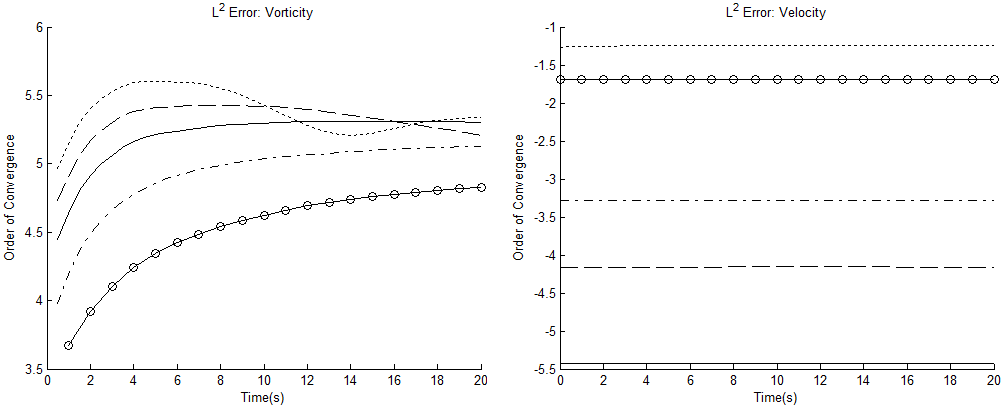
\includegraphics[width=1\textwidth]{CutoffWU.PNG}
\caption{\label{fig:CutoffWU}Comparison of convergence effects on vorticity and velocity by kernel cutoff radius for $\delta/\Delta x$=0.1($\cdot \cdot \cdot$), 0.2(--{ }--), 0.3(---), 0.5(--\,$\cdot$\,--), 0.9(--\!$\ominus$\!--);  Perlman vortex, sixth order method.}
\end{figure}

\subsubsection{Convergence Rates of Various Orders}
A 3rd through 6th order method was used to measure convergence rate for various orders; the 6th order method has identical solver parameters as that used in the cutoff radius experiments. Figure \ref{fig:Porder} provides a comparison of the observed convergence rate of the vorticity for each of the various order methods. The 3rd and 4th order methods converge at full order, while the 5th and 6th order solutions converge at a little more than one half of an order less than optimal.

\begin{wrapfigure}{R}{.52\textwidth}
\centering
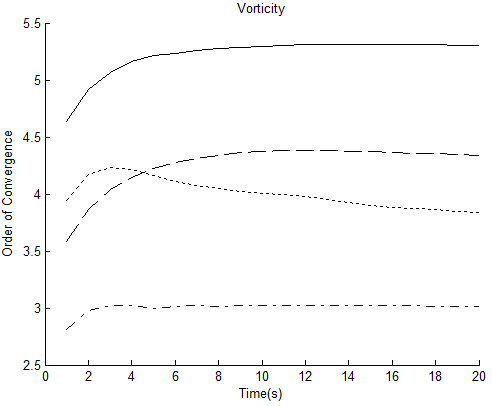
\includegraphics[width=0.52\textwidth]{PorderR.PNG}
\caption{\label{fig:Porder}Comparison of convergence rate for various order methods: 3rd(--\,$\cdot$\,--), 4th($\cdot \cdot \cdot$), 5th(--{ }--), and 6th(---), Perlman vortex.}
\end{wrapfigure}

\subsubsection{Invariance of Conserved Quantities}\label{PConserveW}
One of the main advantages of the velocity-vorticity form is explicit conservation of vorticity. The left plot in Figure \ref{fig:PW_LinImpconserve} plots the log of relative conservation of vorticity with respect to initial total vorticity at t=0. Similar to total vorticity, moments of vorticity should also be conserved. The first moment, linear impulse can provide a useful diagnostic to check the validity of the solution. The right plot in Figure \ref{fig:PW_LinImpconserve} plots the total linear impulse for the sixth order method with varying numbers of elements. It is conserved to within nearly machine precision; solutions with more elements actually display a decrease in conservation of linear impulse, which is likely a result of a higher rate of accumulation of roundoff errors due to the greater number of degrees of freedom.

\begin{figure}
\centering
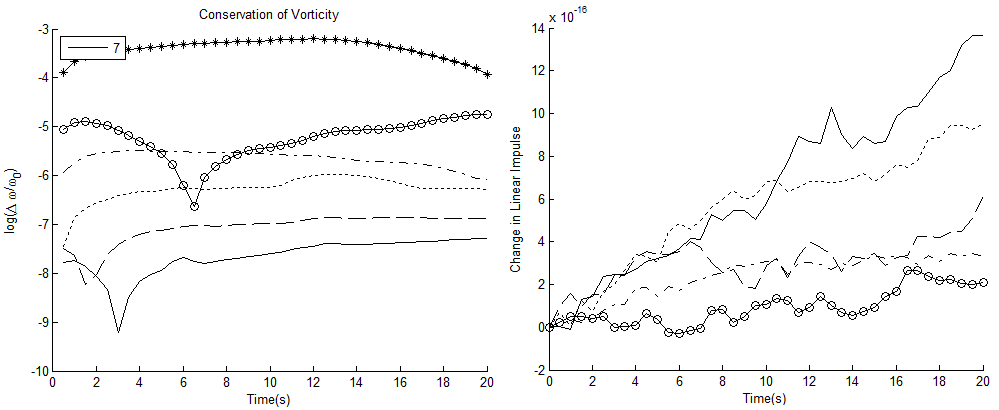
\includegraphics[width=1\textwidth]{PW_LinImpconserve.png}
\caption{\label{fig:PW_LinImpconserve}Conservation of total vorticity (left) and linear impulse (right), Perlman test case, sixth order method with K$\times$K elements K= 3((--\!$\ominus$\!--), 4(--\,$\cdot$\,--), 5($\cdot \cdot \cdot$), 6(--{ }--), and 7(---).}
\end{figure}

%---------
\subsection{Strain: Interacting Vortex Patches}
Strain's system of interacting random vortex patches \cite{Strain1996} forms the next validation case. Specific initial conditions are specified for each of the vortex patches in Table \ref{table:StrainTable} with the overall system consisting of the linear superposition of each patch
\ben{StrainV} \omega(x,y,0) = \sum_{j=1}^m \Omega_j exp(-((x-x_j)^2 + (y-y_j)^2)/\rho_j^2) \ee
An explicit data set for the results is not reported, but a set of contour plots illustrates the time evolution. The same parameters are used in the present solver and similar contour plots are compared against the validating set.

\begin{table}
\centering
\caption{Interacting Vortex Patch Parameters}\label{table:StrainTable}
\begin{tabular}{lllll}
\hline
j & $x_j$    & $y_j$    & $\rho_j$ & $\Omega_j$ \\ \hline
1 & -0.6988 & -1.7756 & 0.6768  & -0.4515   \\
2 & 1.4363  & -1.4566 & 0.3294  & 0.4968    \\
3 & -0.1722 & 0.4175  & 0.5807  & -0.9643   \\
4 & -1.5009 & -0.0937 & 0.2504  &  0.3418    \\ \hline
\end{tabular}
\end{table}

\subsubsection{Comparison with Originally Published Results}\label{SComp}
Although an analytical solution does not exist for the given vortex system, we shall compare the solution from the present method with that obtained by Strain \cite{Strain1996}. He does not note the contour intervals used in the creation of his plots, but the strength and location of the initial vorticity patches are known. From this a digital scan of his initial vorticity plot was used to determine the radial distance of each contour line, and then the vorticity evaluated according to \eqref{StrainV} at the radial distance of the contour line. Based on this the approximate contour intervals determined were (-0.831, -0.696, -0.563, -0.43, -0.3, -0.168, -0.032, 0.099, 0.227, 0.364).

Figure \ref{fig:StrainComp} provides a qualitative comparison of a sixth order method solution with Strain's results at t=28. The two sets of results agree very well. Notably, the solution from the current method with only approximately 3000 degrees of freedom replicates quite well Strain's result where N=25600. In all convergence test cases vorticity was conserved to within 0.03\% and linear impulse to within 2E-5.
\begin{figure}[t]
\centering
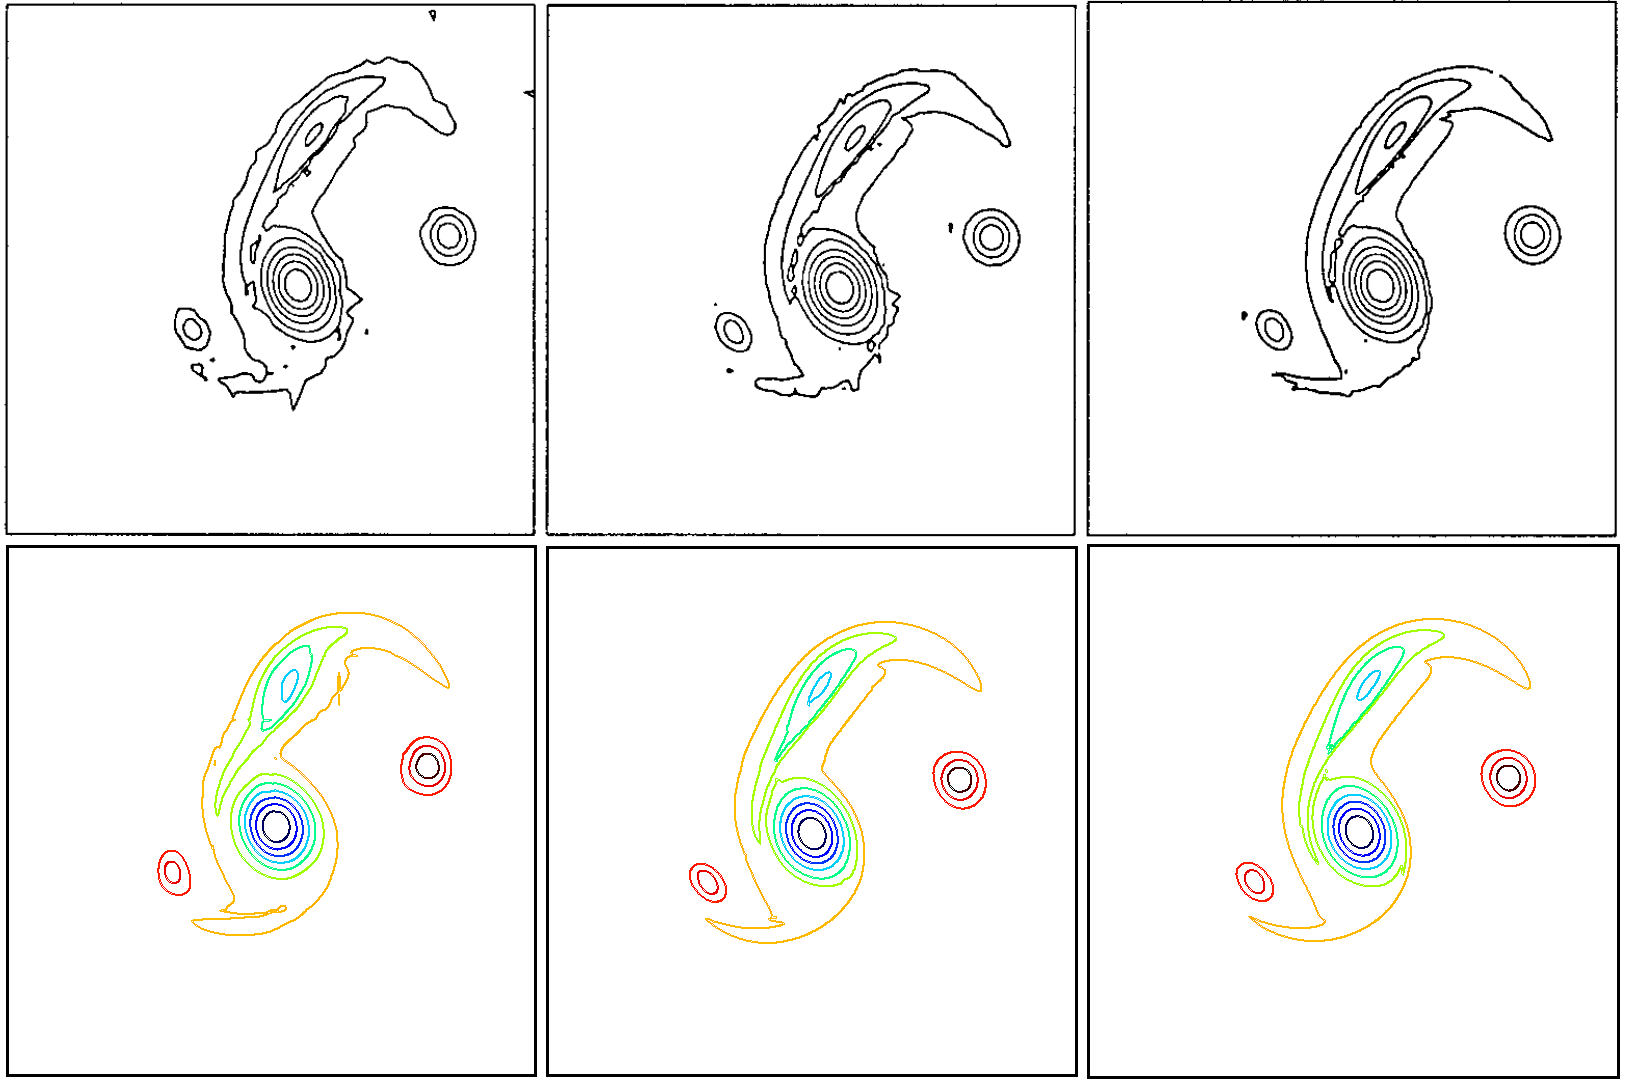
\includegraphics[width=1\textwidth]{StrainCompRmod.PNG}
\caption{\label{fig:StrainComp}Comparison of Strain \cite{Strain1996} (left) with present method (right) t=28. Left to right, top to bottom: DOF= 6400, 12800, 25600; 3136, 7056, 63504. Contour interval for right column specified in \S\ref{SComp}. Reprinted with permission \cite{StrainLic}. }
\end{figure}

\subsubsection{Approximated Convergence Rates of Various Orders}\label{SConverge}
In order to be able to make a quantitative comparison lower degree of freedom solutions were compared against a pseudo-exact solution with far more elements. The error in the higher degree of freedom solution with respect to an exact solution should be dwarfed by the error of the lower degree of freedom solutions. In this case a sixth order 60$\times$60 element solution was used as the comparative solution. A time-step of $\Delta t=0.32$ was chosen to satisfy the CFL condition in all tests allowing the time-step to be kept constant across all tests.

A set of lower element count sixth order runs were performed with two different cutoff radii. There is a striking difference in the convergence properties of each. Early on the smaller cutoff radius run displays superior convergence, but this continually decays over time. The convergence rate is poorer initially for the larger cutoff radius result, but it remains fairly steady at a 3rd order convergence. The convergence rate behavior is to be expected given the results of the Perlman cutoff radius tests. The larger cutoff radius lowers the convergence rate of the calculated velocity field (and therefore the overall method), but the accumulated quadrature error over time is much smaller, enough that the convergence rate is relatively steady.

\begin{wrapfigure}{R}{.5\textwidth}
\centering
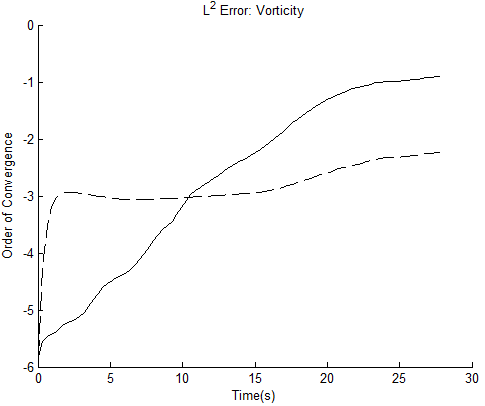
\includegraphics[width=.5\textwidth]{Strain6vs6R.PNG}
\caption{\label{fig:Strain6vs6}Dependency of rate of convergence on cutoff radius in sixth order method, for a $\delta/\Delta x$= 0.5(--{ }--) and 0.25(---), Strain vortex patches. }
\end{wrapfigure}

%---------
\subsection{Koumoutsakos: Elliptical Vortex}
The final validation case is the evolution of an elliptical vortex patch \cite{Koum1997}. The specific initial configuration is specified as
\be \omega^{II}(r) = 20(1-(r/0.8)^4), \; r\leq 0.8 \quad \omega^{II}(r)=0, \; r>0.8 \ee
however the cases tested were actually elliptical, to accommodate this the initial distribution was modified to
\ben{KoumEqn} \omega^{II}(x,y,0)_{mod} = 20(1-((x/a)^2+(y/b)^2)^2/0.8^4 ) \quad a=1, \; b=2 \ee
The contour levels are specified in the resultant figure as 0.25, 0.50, 1, 2, ..., 20; these levels are used in the current code's resultant plot for direct comparison.

\subsubsection{Comparison with Originally Published Results}\label{KoumComper}
Although an analytical solution does not exist for the given vortex system, we shall compare the solution from the present method with that obtained by Koumoutsakos \cite{Koum1997}. Identical contour intervals were used and the solution was observed at similar times. The smoothness of the initial vorticity configuration is limited by the polynomial generating function, so a 4th order method was used with $30^2$ elements and a $\delta/\Delta x=0.4$. In order to satisfy the CFL condition a time-step of 0.0104 seconds was necessary.

Figures \ref{fig:KoumComp1} and \ref{fig:KoumComp2} compare the evolution of the solution obtained from the present method with the results of Koumoutsakos. With the exception of some numerical artifacts near regions of strong vorticity gradients, all of the plots agree quite well.

It is uncertain whether the third observation time reported by Koumoutsakos is rounded \cite{Koum1997}, it does not match up with the expected vortex behavior. All other matching times occurred within a tenth of a second of the reported time, reasonably explained by rounding.

\begin{figure}[t]
\centering
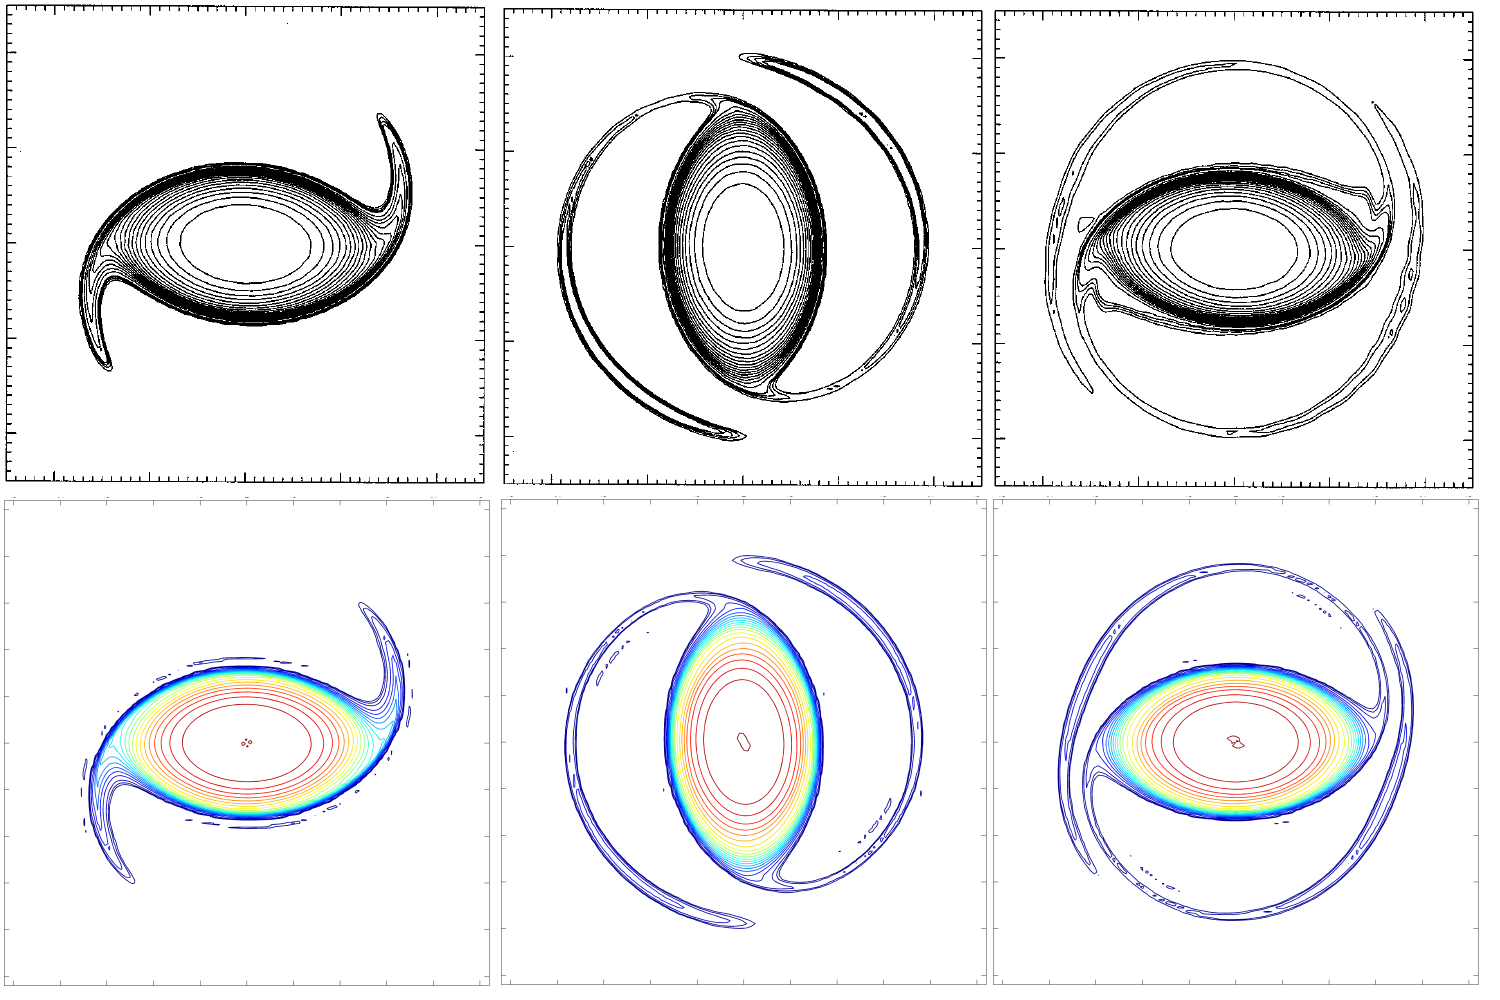
\includegraphics[width=1\textwidth]{KoumComp1R.PNG}
\caption{\label{fig:KoumComp1}Comparison of vorticity, Koumoutsakos \cite{Koum1997} (top) and present method (bottom). From left to right, top to bottom: t=1, 2, 4; 0.80, 1.93, 2.32. Reprinted with permission \cite{KoumLic}.}
\end{figure}
\begin{figure}[t]
\centering
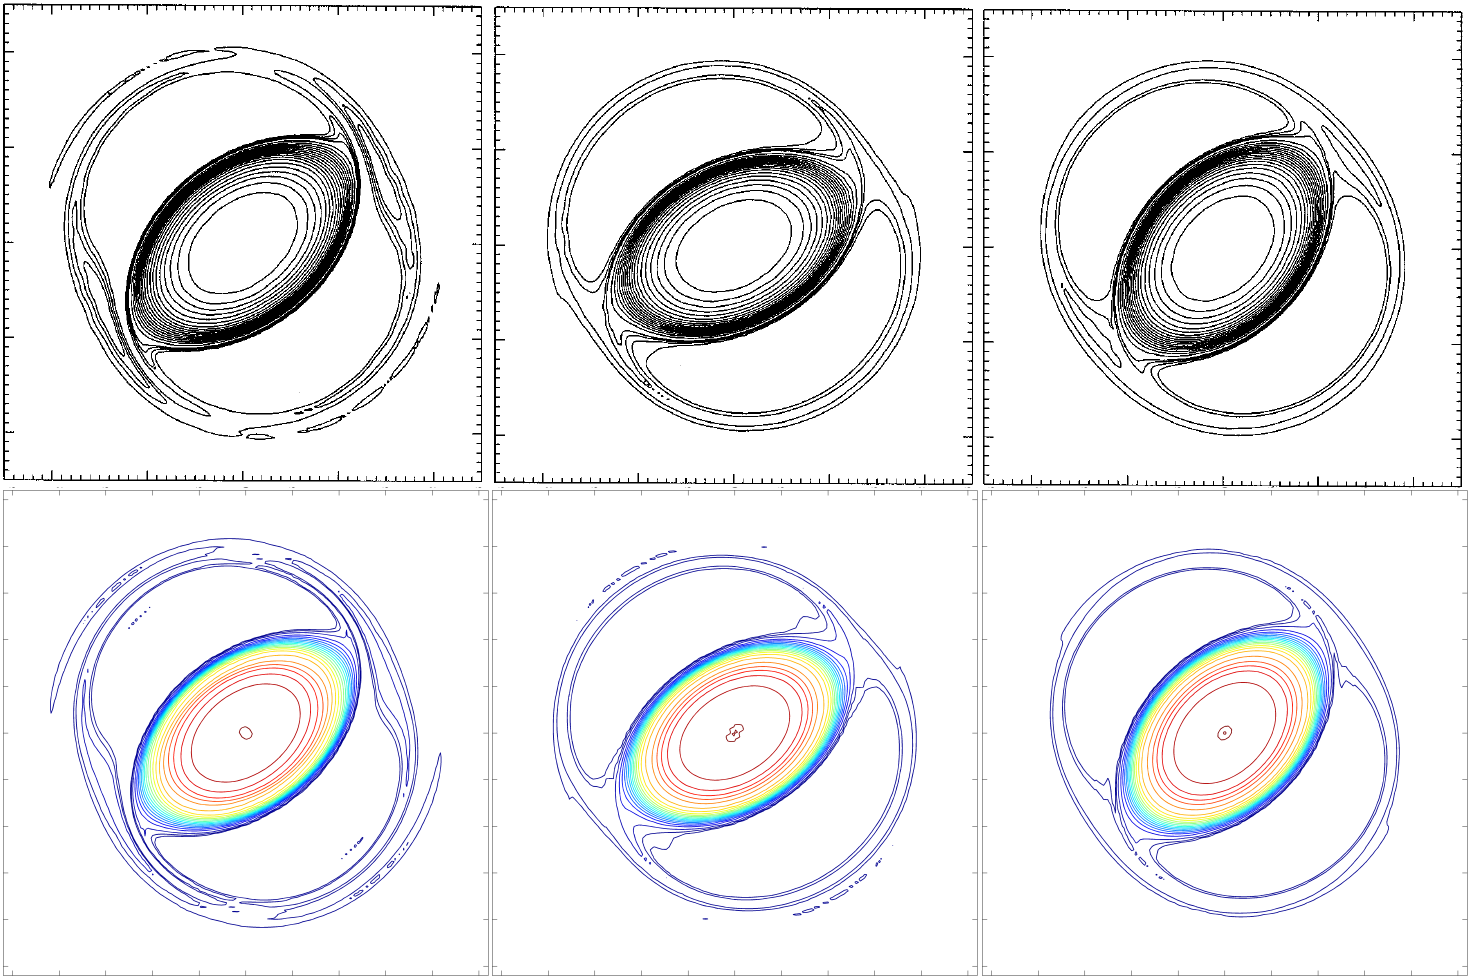
\includegraphics[width=1\textwidth]{KoumComp2R.PNG}
\caption{\label{fig:KoumComp2}Comparison of vorticity, Koumoutsakos \cite{Koum1997} (top) and present method (bottom). From left to right, top to bottom: t=6, 12, 18; 5.94, 11.99, 17.94. Reprinted with permission \cite{KoumLic}.}
\end{figure}

%
\subsubsection{Evolution of Aspect Ratio}
One important feature of the test case studied by Koumoutsakos \cite{Koum1997} was its non-axisymmetrization. The time evolution of the ellipticity was monitored by observing the change of the effective aspect ratio with respect to time. This provides an additional method of comparison between the results of the present method and  those of Koumoutsakos.

Figure \ref{fig:AspectRatio} compares the evolution of the two effective aspect ratios, the solver parameters were identical to those used in \S\ref{KoumComper}. The plots agree well, the most pronounced difference being the greater amplitude of the peaks in the quasi-steady state for $t>17$ compared to Koumoutsakos' results.
\begin{figure}
\centering
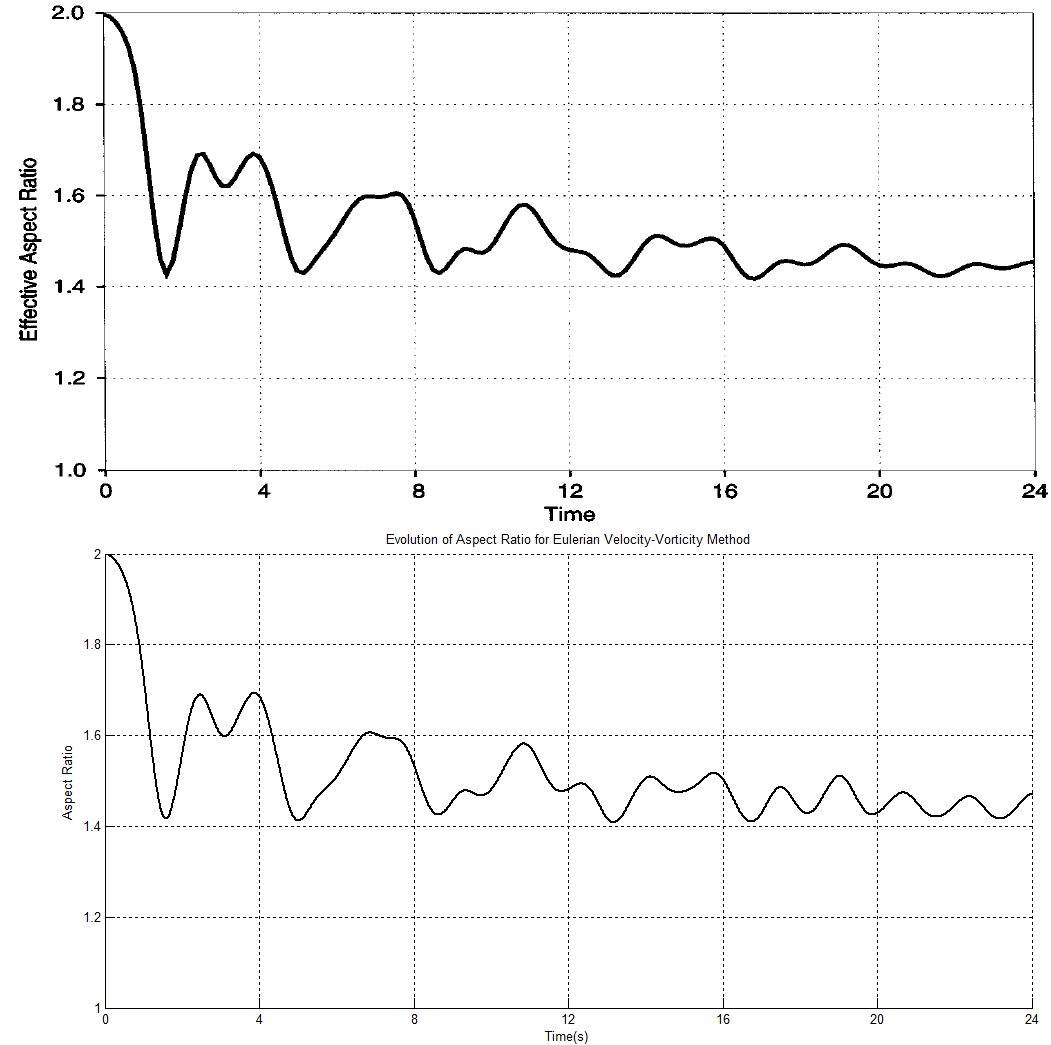
\includegraphics[width=1\textwidth]{AspectRatio.PNG}
\caption{\label{fig:AspectRatio}Comparison of effective aspect ratio, Koumoutsakos \cite{Koum1997} (top) and present method (bottom). Reprinted with permission \cite{KoumLic}.}
\end{figure}\\

%============================================================
\section{Pending Improvements: Exact Biot-Savart Evaluation via Modified Kernel }

Ideally one would exactly integrate the Biot-Savart kernel, removing both the quadrature error from poor convergence for a nearly-singular kernel and the approximation error in de-singularizing the kernel. For example, should one wish to calculate the y-velocity at a target point $T_x$ the following must be evaluated:
\be u_y(T_x) = \int \int \frac{\mathbf{x}-T_x}{2\pi r^2} \omega(\mathbf{x}) d\mathbf{x} \ee
where the vorticity, $\omega$, is actually a Lagrange interpolation. Thus:
\be u_y(T_x) = \frac{1}{2 \pi} \sum_i \sum_j z_{ij} \int \int \frac{x-T_x}{r^2} \; \ell_i(x) \ell_j(y) \;dx \;dy\ee
ehre $z_{ij}$ is the value of the vorticity interpolation at the $i,j$ node.

Notably the variable portion of the interpolation, the interpolatory values, occur outside of the integral since the interpolation is a linear combination of each of the Lagrange bases. This permits pre-calculation and storage of the integral values by an accurate method of choice without worrying about its impact on the runtime performance of the actual simulation. With a method of suitable accuracy to calculate these integrals the runtime calculation of the velocity can be made to agree to within machine precision of the exact value. The storage and use of pre-calculated values yields a modified numerical quadrature routine with special weights of the form:

\be u(T_-)= \frac{1}{2 \pi} \sum_i \sum_j z_{ij} W_{(-, T_x,T_y,i,j)} \ee
where the special weights range over each coordinate direction, target evaluation positions, and source interpolation point positions respectively.

One important consideration is what is the spatial variance of these special weights with respect to the source interpolation points. To examine this heuristically one may divide the special quadrature weights by the standard weights obtained from the tensor product of the Gauss-Legendre interpolation points used. For simplicity consider this case for a single target point and velocity in the x-direction:
\be u_x= \frac{1}{2 \pi} \sum_i \sum_j z_{ij} \frac{W_{(i,j)}}{W_{GL}} W_{GL} \ee
where we have denoted the outer product of the Gauss-Legendre quadrature weights along each direction as $W_{GL}$.

Note that $z_{ij}$ is only the interpolatory values of the vorticity, it is not linked in any way to the value of the Biot-Savart kernel values which also vary spatially. If the special quadrature weights are able to exactly evaluate the velocity, the factor $\overset{\sim}{k}_{ij} = \frac{W_{(i,j)}}{W_{GL}}$ may be thought of as a modified kernel value at each interpolatory point so that one recovers a more familiar form:
\be u_x= \frac{1}{2 \pi} \sum_i \sum_j z_{ij}  \overset{\sim}{k}_{ij} W_{GL} \ee
which is identical to the naive approach of evaluating the Biot-Savart integral with Gauss-Legendre quadrature, however it is able to exactly evaluate the integral thanks to the modified kernel values.

Now that we have recovered a set of modified kernel values we can examine their spatial variance. Figure \ref{fig:KernelModComp} plots the relative variance of the modified kernel values with respect to the traditional Biot-Savart kernel values for a 6th order method with a target point at the center of an element across the ``self'' element and the adjacent elements along one coordinate direction. Within the self element there is significant difference between the two sets of kernel values, however this decays as one moves farther away from the target point. For elements farther away than this the absolute difference between the two sets of kernel values differs to within machine precision.

This presents several fortunate consequences; one need only pre-calculate modified kernel values for the self and adjacent elements. Additionally, the kernel values need only be modified locally which presents promising opportunity for the application of a Fast Multipole Method. This exact Biot-Savart evaluation technique is currently in development for use in the current overall solution method and it is expected that with proper application significant gains in the overall convergence of the method will be realized.

\begin{figure}
\centering
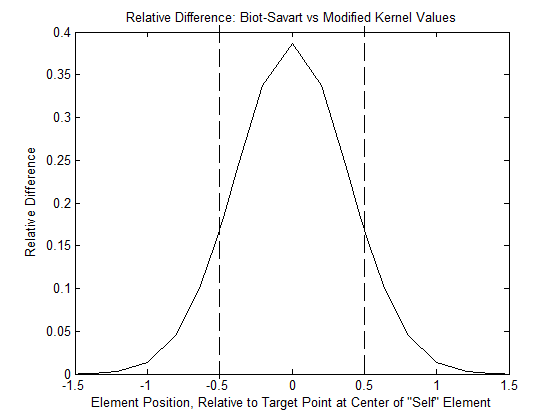
\includegraphics[width=.6\textwidth]{KernelModComp.PNG}
\caption{\label{fig:KernelModComp}Spatial variance of modified Biot-Savart kernels compared to that of tradition kernel values along a coordinate direction for a particular target point at the center of an element for a 6th order interpolation scheme}
\end{figure}

%============================================================
\section{Conclusion}

A complete high-order method for velocity-vorticity inviscid flow that integrates all necessary subsystems was created. Both the solver and the underlying Eulerian vortex approach were validated against analytical and qualitative test cases. Finally, the $L^2$ error, vortex diagnostics, and convergence rate were measured. The method was shown capable of achieving near optimal convergence rate in the analytical test case. In flows where vorticity is changing rapidly spatially the method suffers from insufficient Biot-Savart quadrature convergence, but still has the possibility of high-order convergence if parameters are chosen carefully. If an improvement were to be made to the ability of the quadrature routine to integrate either the nearly singular Biot-Savart kernel approximation or to directly handle the singular kernel it may be possible to maintain near-optimal overall convergence of the method without decay over time.

%============================================================
%\section*{Acknowledgments}

%============================================================
\newpage
\begin{thebibliography}{9}% maximum number of references (for label width)
%Me!
\bibitem{Bevan}
Bevan, J. J., \textit{Vortex Dominated Flows: A High-order, Conservative Eulerian Simulation Method}. Master's Thesis, University of Massachusetts Lowell, 2015.

%VortexRefs
\bibitem{Saffman1992}
Saffman P. G., \textit{Vortex Dynamics}, Cambridge Univ. Press, Cambridge, UK, 1992.
\bibitem{Rosenhead1930}
Rosenhead L., "The spread of vorticity in the wake behind a cylinder," \textit{Proc. Roy. Soc. London Ser. A}, Vol. 127, 1930, pp. 590.
\bibitem{Moore1972}
Moore D. W., "Finite amplitude waves on aircraft trailing vortices," \textit{Aero. Quart.}, Vol. 23, 1972, pp. 307.

%VortexMeths
\bibitem{Point4}
Chorin A. J., Bernard P. S., "Discretization of a vortex sheet, with an example of roll-up," \textit{J. Comput. Phys.}, Vol. 13, No. 3, 1973, pp. 423-429.
\bibitem{Line4}
Leonard A., \textit{Numerical simulation of interacting, three-dimensional vortex filaments}, in: \textit{Proceedings of the IV Intl. Conference on Numerical Methods of Fluid Dynamics}, no. 35 in \textit{Lecture Notes in Physics}, Springer-Verlag, 1975, pp. 245-250.
\bibitem{Sheet1}
Agishtein M. E. , Migdal A. A., "Dynamics of vortex surfaces in three dimensions: Theory and simulations," \textit{Physica D}, Vol. 40, 1989, pp. 91-118.
\bibitem{Volumes1}
Russo G., Strain J. A., "Fast triangulated vortex methods for the 2D Euler equations," \textit{J. Comput. Phys.}, Vol. 111, 1994, pp. 291-323.

%VortexAux
\bibitem{Strain1997}
Strain J., "Fast adaptive 2D vortex methods," \textit{Journal of computational physics}, Vol. 132, No.1, 1997, pp. 108-122.
\bibitem{LindsayKrasny2001}
Lindsay K., and Krasny R., "A particle method and adaptive treecode for vortex sheet motion in three-dimensional flow," \textit{J. Comput. Phys.}, Vol. 172, No.2, 2001, pp. 879-907.
\bibitem{WL}
Winckelmans, G. S., Leonard A., "Contributions to vortex particle methods for the computation of three-dimensional incompressible unsteady flows," \textit{J. Comput. Phys.}, Vol. 109, No. 2, 1993, pp. 247-273.
\bibitem{BealeMajda}
Beale, J. T., and Majda A., "High order accurate vortex methods with explicit velocity kernels," \textit{J. Comput. Phys.}, Vol. 58, No. 2, 1985, pp. 188-208.

%Remeshing problems
\bibitem{Remesh2}
Beale J. T., "On the accuracy of vortex methods at large times,"  \textit{IMA Workshop on Computational Fluid Dynamics and Reacting Gas Flows}, Springer-Verlag, 1988, p. 19.\bibitem{Remesh3}
Marshall J. S., Grant J. R., "Penetration of a blade into a vortex core: vorticity response and unsteady blade forces," \textit{J. Fluid Mech}, Vol. 306, 1996, pp. 83-109.
\bibitem{Remesh4}
Nordmark H. O., "Rezoning for higher order vortex methods," \textit{J. Comput. Phys.}, Vol. 97, 1991, pp. 366-397.
\bibitem{Remesh5}
Najm H. N., Milne R. B., Devine K. D., Kempa S. N., "A coupled Lagrangian-Eulerian scheme for reacting flow modeling," \textit{ESAIM Proc.} Vol. 7, 1999, pp. 304-313.

%Brown
\bibitem{Brown2000}
Brown R.E., "Rotor Wake Modeling for Flight Dynamic Simulation of Helicopters," \textit{AIAA Journal}, Vol. 38, No. 1, 2000, pp. 57-63.
\bibitem{Brown2004}
Line A.J., BrownR.E., "Efficient High-Resolution Wake Modelling using the Vorticity Transport Equation," \textit{60th Annual Forum of the American Helicopter Society}, Baltimore, MD, 2004.

%DG
\bibitem{HestWar}
Hesthaven, J. S. and Warburton, T., \textit{Nodal discontinuous Galerkin methods}, Vol. 54 of \textit{Texts in Applied Mathematics}, Springer, New York, 2008, Algorithms, analysis, and applications.
\bibitem{RKDG}
Cockburn, B. and Shu, C.-W., “Runge-Kutta discontinuous Galerkin methods for convection-dominated problems,” \textit{J. Sci. Comput.}, Vol. 16, No. 3, 2001, pp. 173–261.

%LSERK
\bibitem{Reid}
Atcheson, T., \textit{Explicit Discontinuous Galerkin Methods for Linear Hyperbolic Problems}. Master's Thesis, Rice University, 2013.
\bibitem{Niegemann}
Niegemann, J., Diehl R., and Busch K., "Efficient low-storage Runge–Kutta schemes with optimized stability regions," \textit{J. Comput. Phys.}, Vol. 231, No. 2, 2012, pp. 364-372.

%Test cases
\bibitem{Perlman1985}
Perlman M., "On the accuracy of vortex methods," \textit{J. Comput. Phys.}, Vol. 59, 1985, pp. 200–223.
\bibitem{Strain1996}
Strain J., "2D vortex methods and singular quadrature rules," \textit{J. Comput. Phys.}, Vol. 124, No. 1, 1996, pp. 131-145.
\bibitem{Koum1997}
Koumoutsakos P., "Inviscid axisymmetrization of an elliptical vortex," \textit{J. Comput. Phys.}, Vol. 138, 1997, pp. 821-857.

%Misc
\bibitem{Persson2013}
Persson P.O., "A Sparse and High-Order Accurate Line-Based Discontinuous Galerkin Method for Unstructured Meshes" \textit{J. Comput. Phys.}, Vol. 233, Jan 2013, pp. 414-429.
\bibitem{MiscMeth1}
Williamson, D. L., "Integration of the barotropic vorticity equation on a spherical geodesic grid," \textit{Tellus}, Vol. 20, No. 4, 1968, pp. 642-653.
\bibitem{MiscMeth2}
Russell, D., and Wang, Z. Jane., "A Cartesian grid method for modeling multiple moving objects in 2D incompressible viscous flow," \textit{J. Comput. Phys.}, Vol. 191, No. 1, 2003, pp. 177-205.
\bibitem{MiscMeth3}
Calhoun, D., "A Cartesian grid method for solving the two-dimensional streamfunction-vorticity equations in irregular regions," \textit{J. Comput. Phys.}, Vol. 176, No. 2, 2002, pp. 231-275.
\bibitem{MiscMeth4}
Suh, J-C. "The evaluation of the Biot–Savart integral. Journal of engineering mathematics," Vol. 37, No. 4, 2000, pp. 375-395.
\bibitem{SteinhoffUnderhill1994}
Steinhoff J., Underhill D., "Modification of the Euler equations for ``vorticity confinement'': Application to the computation of interacting vortex rings," \textit{Phys. Fluids}, Vol. 6, No. 8, 1994, pp. 2738-2743.

%Licenses
\bibitem{KoumLic}
Reprinted from \textit{Journal of Computational Physics}, Vol. 138, Koumoutsakos P., Inviscid axisymmetrization of an elliptical vortex, pp. 821-857, Copyright (1997), with permission from Elsevier.
\bibitem{StrainLic}
Reprinted from \textit{Journal of Computational Physics}, Vol. 124, No.1, Strain J., 2D vortex methods and singular quadrature rules, pp. 131-145, Copyright (1996), with permission from Elsevier.
\end{thebibliography}

\end{document}

% - Release $Name:  $ -
